%! TeX program = lualatex
\documentclass[twoside, a4paper, 12pt]{book}

\title{Geometryczna Teoria Grup}
\author{\color{subtext1}Weronika Jakimowicz}
\date{Zima 2024/25}

\usepackage[dates, pl]{../../../template}

% \includeonly{rozdzialy/07.tex}

\usepackage{halloweenmath}

\begin{document}
\frontmatter 
\maketitle
\thispagestyle{empty}
\setcounter{page}{0}

\tableofcontents
\mainmatter

\pagestyle{fancy}
  
\section{02.10.2024}{Grafy Cayleya}

\subsection{Metryka słów}

\begin{definition}{metryka słów}{}
  Niech $G$ będzie grupą, a $S$ dowolnym układem jej generatorów. Wówczas dla dowolnych $g_1,g_2\in G$ \buff{odległość między nimi w metryce słów} definiujemy jako
$$ds(g_1, g_2)=\min\{n\;:\;g_2=g_1s_1,...,s_n,\;s_i\in S\cup S^{-1}\},$$
gdzie $S^{-1}=\{g^{-1}\;:\;g\in S\}$.
\end{definition}

Metryka słów jest 
\begin{enumerate}
  \item skończona
  \item symetryczna (z definicji generatorów)
  \item \hl{lewo-niezmiennicza}, czyli $(\forall\;\gamma\in G)\;ds(\gamma g_1,\gamma g_2)=ds(g_1, g_2)$
\end{enumerate}
Ostatnia własność oznacza, że $G$ działa na sobie jako na przestrzeni metrycznej przez izometrie.

Gromov chce patrzeć na dyskretne przestrzenie metryczne, jakimi są grupy z metryką słów, jako na przestrzenie ciągłe (z dużej odległości).

\subsection{Graf Cayleya}

\begin{definition}{graf Cayleya}{}
Niech $G$ będzie grupą, a $S$ zbiorem jej generatorów. $C(G, S)$ to graf Cayleya o wierzchołkach będących elementami $G$ i skierowanych krawędziach etykietowanych generatorami:
\begin{center}
  \begin{tikzcd}
    g\arrow["s", r] & gs
  \end{tikzcd}
\end{center}
gdzie $g\in G$ i $s\in S$.
\end{definition}

\begin{example}[m]
\item Dla $G=\Z^2$ oraz $S=\{{\color{red}\overbrace{(1, 0)}^s}, {\color{blue}\overbrace{(0, 1)}^t}\}$ graf Cayleya to nieskończona "kratka"
  \bigskip

  \begin{center}
    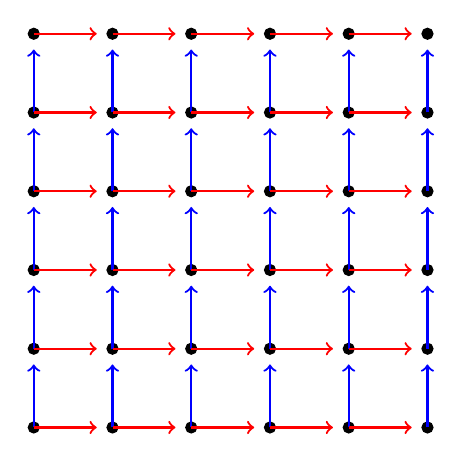
\begin{tikzpicture}
      \foreach \x in{0,...,5} { 
        \foreach \y in{0,...,5} {
          \filldraw (\x, \y) circle (2pt);
        }
      }

      \foreach \x in {0,...,5} {
        \foreach \y in {0,..., 4} {
          \draw[->, blue, thick] (\x, \y) -- (\x, \y+.8);
        }
      }
      \foreach \x in {0,...,4} {
        \foreach \y in {0,..., 5} {
          \draw[->, red, thick] (\x, \y) -- (\x+.8, \y);
        }
      }
    \end{tikzpicture}
  \end{center}
\item Dla grupy cyklicznej rzędu $p$ z generatorem $\color{red}s$ graf Cayleya to $p$-kąt
  \begin{center}
    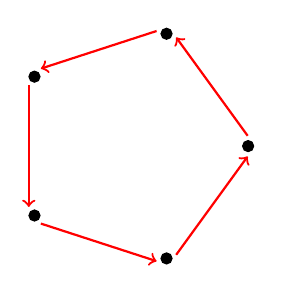
\begin{tikzpicture}
      \foreach \i in {0,..., 4} {
        \filldraw ( 360 /5 * \i :1.5) circle (2pt);
        \draw[->, red, thick] (360/5*\i + 5:1.5) -- (360/5*\i + 360/5 - 5:1.5);
      }
    \end{tikzpicture}
  \end{center}
\item {\color{red}\Large TO DO} parkietarz kwadratami
\end{example}

Każdy graf Cayleya jest \buff{spójny}, bo jego krawędzie to mnożenie przez generatory. Dodatkowo, grupa $G$ działa na nim przez \hl{automorfizmy zachowując krawędzie oraz ich etykiety}. To znaczy, że krawędż z wierzchołkami \begin{tikzcd}g\arrow[r, "s"]&gs\end{tikzcd} pod działaniem elementu $\gamma \in G$ staje się \begin{tikzcd}\gamma g\arrow[r, "s"] & \gamma gs\end{tikzcd}.

Jeśli każdą krawędź w grafie Cayleya potraktujemy jako odcinek długości $1$, to możemy na nim zdefiniować metrykę która jako odległość dwóch punktów przyjmuje długość najkrótszej ścieżki między nimi. Ta metryka na wierzchołkach pokrywa się z \buff{metryką słów} na grupie $G$ o generatorach $S$, której graf rozpatrujemy. Przy takiej metryce działanie grupy $G$ jest więc działaniem nie tylko przez automorfizmy, ale przez izometrie (lewa-niezmienniczość).


\section{25.02.2025}{Produkty i koprodukty kategorii}

\subsection{O obiektach początkowych i końcowych słów kilka}

\begin{definition}{obiekt początkowy i końcowy}{}
  Powiemy, że obiekt $C\in \Cc_0$ jest \buff{początkowy}, jeśli dla każdego $D\in\Cc_0$ istnieje dokładnie jeden morfizm $C\to D$, $|\Cc(C, D)|=1$. Analogicznie definiujemy \buff{obiekt końcowy} $C$: $\forall\;D\in\Cc_0\;|\Cc(D, C)|=1$.
\end{definition}

\begin{example}[m]
  \item W kategorii, której obiektami jest odcinek $\Cc_0=[0,1]$, a morfizmy to relacja $\leq$ obiektem początkowym jest $0$, a końcowym - $1$.
  \item W kategorii zbiorów obiektem początkowym jest $\emptyset$, a obiektem końcowym jest singleton.
  \item W $Gr$ grupa trywialna jest zarówno obiektem początkowym jak i końcowym.
  \item Kategoria, która ma dwa obiekty bez morfizmów między nimi nie ma obiektu końcowego ani początkowego.
\end{example}

\begin{fact}{}{}
  Obiekty końcowe i początkowe, jeśli istnieją, to są jedyne z dokładnością do izomorfizmu.
\end{fact}

\begin{proof}
  Niech $C$ i $C'$ będą obiektami końcowymi kategorii $\Cc$. Wiemy, że $\Cc(C, C)=\{id_C\}$, czyli komutujący diagram
  \begin{center}
    \begin{tikzcd}
      C \arrow[rr, "id_C"]\arrow[dr, "\exists!f" below left] & & C\\ 
                           & C'\arrow[ur, "\exists!g" below right]
    \end{tikzcd}
  \end{center}
  daje $g\circ f=id_C$. Analogiczny diagram daje $f\circ g=id_{C'}$. Stąd $f$ i $g$ to para wzajemnie odwrotnych izomorfizmów między $C$ i $C'$
\end{proof}

\subsection{(Ko)granice funktorów a (ko)produtky}

Niech $F:\mathcal{I}\to \Cc$ będzie funktorem, gdzie o kategorii $\mathcal{I}$ myślimy jako o kategorii indeksów. Przez $\Cc^{\mathcal{I}}$ oznaczmy kategorię wszystkich takich funktorów. 
Powiemy, że funktor $C$ jest stały, jeżeli $C(i)=C$ dla każdego $i\in\mathcal{I}_0$ oraz $C(f)=id_C$ dla każdego morfizmu.

Budujemy kategorię, której 
\begin{itemize}
  \item obiekty to wszystkie naturalne przekształcenia funktora $F$ w funktory stałe $C$, $\phi:F\implies C$, czyli komutujące diagramy (kostożki) 
    \begin{center}
      \begin{tikzcd}
        F(i)\arrow[rr, "F(f)"]\arrow[dr, "\phi_i" below left] & & F(j)\arrow[dl, "\phi_j"]\\ 
                                                  & C
      \end{tikzcd}
    \end{center}
  \item a morfizmy to strzałki $C\to D$ takie, że diagram
    \begin{center}
      \begin{tikzcd}
        C\arrow[rr] & & D\\ 
                    & F\arrow[ur, Rightarrow, blue, "\phi" below right]\arrow[ul, Rightarrow, orange, "\psi" below left]
      \end{tikzcd}
    \end{center}
    komutuje.
\end{itemize}

Diagram wyżej można rozpisać jako:
\begin{center}
  \begin{tikzcd}[column sep=large]
    & F(i)\arrow[d] \arrow[ddl, "\phi_i" above left, blue]\arrow[ddr, "\psi_i" above right, orange] \\ 
    & F(j)\arrow[dl, "\phi_j" above, blue]\arrow[dr, "\psi_j" above, orange]\\ 
    D & & C\arrow[ll]
  \end{tikzcd}
\end{center}

\begin{definition}{kogranica funktora}{}
  \buff{Kogranicą} (\acc{granica prosta}) funktora $F$, $\varinjlim F$, nazywamy obiekt początkowy w wyżej zdefiniowanej kategorii naturalnych przekształceń. 
  % \buff{Granica} (\acc{granica odwrotna}) to wtedy obiekt końcowy powyższej kategorii ze wszystkimi strzałkami zdualizowanymi $\varprojlim F$.
\end{definition}

Diagram wyżej możemy zdualizować i zamiast rozpatrywać naturalne przekształcenia $\phi:F\implies C$ możemy rozważyć naturalne przekształcenia $\phi:C\implies F$, czyli diagramy (stożki)
\begin{center}
  \begin{tikzcd}
    & C \arrow[dl, "\phi_i" above left] \arrow[dr, "\phi_j" above right]\\ 
    F(i)\arrow[rr, "F(f)" below] & & F(j)
  \end{tikzcd}
\end{center}
z morfizmami {definiowanymi analogicznie. 

\begin{definition}{granica funktora}{}
  \buff{Granica} (\acc{granica odwrotna}) to obiekt końcowy powyższej kategorii stożków, $\varprojlim F$.
\end{definition}

% {\color{red}tutaj jest zdjecie
%
% przyklad dla kategorii zbiorów
%
% ja chyba chce wziąć dwuelementową kategorię $\mathcal{I}$ i tutaj policzyć, jeśli $F(1)=G$, a $F(2)=H$.
% }
%
Rozważmy kategorię $\mathcal{I}$, która ma dwa obiekty $\mathcal{I}_0=\{0,1\}$. Niech $F:\mathcal{I}\to Set$ będzie funktorem, dla którego $F(0)=A$, a $F(1)=B$. Niech $\phi$ oraz $\psi$ będzie parą naturalnych przekształceń, dla których
\begin{center}
  \begin{tikzcd}[column sep=large, row sep=large]
     & \varinjlim F\arrow[dl, "\phi_0" above left] \arrow[dr, "\phi_1"] \\ 
    F(0)=A & D \arrow[l, "\psi_0"] \arrow[r, "\psi_1" below right] \arrow[u, "\exists!f", dashed] & F(1)=B
  \end{tikzcd}
\end{center}
gdzie pionowa strzałka istnieje i jest jedyna, bo $\varinjlim F$ to obiekt końcowy. Jeśli weźmiemy $\varinjlim F=A\times B$, a $\phi_0=\pi_A$ oraz $\phi_1=\pi_B$ będą rzutami i $f(d)=(\psi_0(d), \phi_1(d))$, to diagram nadal jest prawdziwy. 

Granica odwrotna tego samego funktora, to z kolei suma rozłączna $A\sqcup B$, bo diagram
\begin{center}
  \begin{tikzcd}[column sep=large, row sep=large]
    F(0)=A\arrow[r, "\psi_0"]\arrow[dr, "\phi_0=i_A" below left] & D & F(1)=B\arrow[l, "\psi_1" above]\arrow[dl, "\phi_1=i_B"]\\ 
                                                       & \varprojlim F= A\sqcup B \arrow[u, dashed, "\exists!f"]
  \end{tikzcd}
\end{center}
gdzie $f(x)=\phi_0(x),$ jeśli $x\in A$ oraz $f(x)=\psi_1(x)$ jeśli $x\in B$, komutuje.

\begin{definition}{(ko)produkt}{}
  \buff{Produktem} obiektów $A$ i $B$ kategorii $\Cc$ nazywamy granicę prostą (kogranicę) funktora $F:\mathcal{I}\to \Cc$ dla $\mathcal{I}$ oraz $F$ jak wyżej.

  \buff{Koproduktem} obiektów $A$ i $B$ kategorii $\Cc$ nazywamy granicę odwrotną (granicę) funktora $F:\mathcal{I}\to\Cc$
\end{definition}

\begin{example}[m]
  \item W kategorii grup produkt to iloczyn kartezjański dwóch grup, tak jak w kategorii zbiorów, tj. dla grup $A,G,H$ komutuje diagram
    \begin{center}
      \begin{tikzcd}[column sep=large, row sep=large]
        & G\times H\arrow[dl, "\pi_G" above left]\arrow[dr, "\pi_H"]\\ 
        G & A\arrow[l, "g"]\arrow[r, "h"]\arrow[u, "g\times h" below] & H
      \end{tikzcd}
    \end{center}
    Koprodukt to z kolei produkt wolny tych dwóch grup:
\begin{center}
  \begin{tikzcd}[column sep=large, row sep=large]
    G\arrow[r, "g"]\arrow[dr, "i_G" below left] & A & H\arrow[l, "h" above]\arrow[dl, "i_H"]\\ 
                                                       & H\ast G \arrow[u, dashed, "\exists!f"]
  \end{tikzcd}
\end{center}
gdzie $f$ nakłada na litery słów $G\ast H$ pochodzące z $G$ morfizm $g$, a na litery pochodzące z $H$ - morfizm $h$.
  \item Niech $F:\mathcal{I}\to (P, \leq)$ z dwuobiektowej kategorii $\mathcal{I}$ w zbiór uporządkowany. Wtedy jeśli mamy diagram 
    \begin{center}
      \begin{tikzcd}
         & \varinjlim F\arrow[dr]\arrow[dl] \\ 
        F(0)=a & d \arrow[l]\arrow[r]\arrow[dashed, u] & F(1)=b
      \end{tikzcd}
    \end{center}
    to znaczy, że $d\leq a$, $d\leq b$ oraz $d\leq \varinjlim{F}$. Żeby więc miało to sens dla dowolnego $d\leq a,b$ to $\varinjlim F=\inf\{a,b\}$. Analogicznie dostajemy, że $\varprojlim F=\sup\{a,b\}$.

  \item Jeśli $\mathcal{I}$ jest kategorią o nieskończenie wielu obiektach bez morfizmów między różnymi obiektami, a $F:\mathcal{I}\to Set$ jest funktorem w kategorię zbiorów, to wówczas kogranicą tego funktora jest nieskończony iloczyn kartezjański $\prod_{i\in\mathcal{I}_0}F(i)$, a granicą - nieskończona suma rozłączna $\bigsqcup_{i\in\mathcal{I}_0}F(i)$.
\end{example}

% kategoria nieskończenie wiele elementów, ale bez strzałek (jako $\mathcal{I}$)
 % Niech $C$ oraz $C'$ będą kogranicami tego samego funktora. Z definicji mamy
% \begin{center}
%   \begin{tikzcd}[column sep=large, row sep=large]
%     & F(i)\arrow[dr, "\phi_i"]\arrow[d, "\psi_i"]\arrow[dl, "\phi_i" above left] \\ 
%     C & C'\arrow[l, "\exists g" above] & C\arrow[ll, bend left=20, "id"] \arrow[l, "\exists f" above]
%   \end{tikzcd}
% \end{center}

\begin{fact}{}{}
  Granica i kogranica funktora, jeśli istnieje, to jest jedyna z dokładnością do izomorfizmu. Stąd również produkty i koprodukty są unikalne.
\end{fact}

\begin{proof}
  Wynika z uniwersalności obiektów końcowych i początkowych.
\end{proof}

% tutaj liczby p-adyczne
% ekwalizator, koekwalizator
%
% \begin{definition}{surjekcja, epimorfizm}{}
%   Jeśli kategoria ma obiekt początkowy równy obiektowi końcowemu...
% \end{definition}

\begin{example}
  Rozważmy funktor $F:\mathcal{I}^{op}\to Grp$, gdzie $\mathcal{I}=(\N, \leq)$ taki, że dla każdych $i,j\in\N$, $i\leq j$ mamy
  \begin{center}
    \begin{tikzcd}[column sep=large]
      F(j)=\Z/p^j\Z\arrow[r, "F(i\to j)=q"] & F(i)=\Z/p^i\Z
    \end{tikzcd}
  \end{center}
  gdzie $q$ to morfizm ilorazowy.

  Liczby $p$-adyczne to rozszerzenie liczb wymiernych różne od liczb rzeczywistych i zespolonych. Całkowite liczby $p$-adyczne to szeregi
  $$\sum_{i=k}^\infty a_ip^i,$$
  gdzie $k\in\N$ oraz $0\leq a_i < p$. Okazuje się, że całkowite liczby $p$-adyczne, $\Z_p$, można zdefiniować jako granicę funktora $F$:
  \begin{center}
    \begin{tikzcd}
      & & \Z_p \arrow[dll]\arrow[dl]\arrow[d]\arrow[drr]\arrow[drrr] \\ 
      ...\arrow[r] & \Z/p^n\Z\arrow[r] & \Z/p^{n-1}\Z\arrow[r] & ... \arrow[r]& \Z/p^2\arrow[r] & \Z/p\Z
    \end{tikzcd}
  \end{center}
\end{example}

\subsection{Obiekty i kategorie monoidalne}

\buff{Monoid} $(M, \star, 1)$ to struktura algebraiczna z binarną operacją oraz elementem neutralnym. Dodatkowo, komutować ma diagram 
\begin{center}
  \begin{tikzcd}
    M^3\arrow[r, "\star\times id"]\arrow[d, "id\times\star" left] & M^2\arrow[d, "\star"]\\ 
    M^2\arrow[r, "\star"] & M
  \end{tikzcd}
\end{center}
co znaczy, że działanie jest łączne.

\begin{definition}{obiekt monoidalny, kategoria monoidalna}{}
  Niech $\Cc$ będzie kategorią z produktem i elementem początkowym. Niech $M\in \Cc$ będzie obiektem, dla którego mamy $\mu:M^2\to M$ oraz $\epsilon: \{1\}\to M$ takie, że komutują diagramy
  \begin{center}
    \begin{tikzcd}[row sep=large, column sep=large]
      M^3\arrow[r, "\mu\times id"]\arrow[d, "id\times \mu" left] & M^2\arrow[d, "\mu"]\\ 
      M^2\arrow[r, "\mu" below] & M
    \end{tikzcd}
  \end{center}
  \begin{center}
    \begin{tikzcd}[row sep=large, column sep=large]
      M\arrow[r, "\epsilon\times id"]\arrow[d, "id\times \epsilon" left]\arrow[dr, "=" above right] & M^2\arrow[d, "\mu"]\\ 
      M^2\arrow[r, "\mu" below] & M
    \end{tikzcd}
  \end{center}
  Wtedy $M$ jest \buff{obiektem monoidalnym}.
  
  Obiekt monoidalny w kategorii $Cat$ nazywa się \buff{kategorią monoidalną}.
\end{definition}

\begin{example}[m]
\item Dowolna kategoria $\Cc$ z koproduktem i obiektem końcowym jest kategorią monoidalna.
\item Kategoria endofunktorów ma strukturę monoidalną. To znaczy, jeśli mamy dwa endofunktory $F, G\in End(\Cc)$, to potrafimy je złożyć w dobry sposób.

  Funktor $T\in End(\Cc)$ oraz dwa naturalne przekształcenia $\mu:T^2\to T$, $\epsilon: Id\to T$, nazywa się \buff{monadą}.
\end{example}

% Czy $S^n\vee S^n$ to produkt czy produkt w kategorii $Toph_\star$. tutaj jakies zdjecie








\section{03.03.2025}{}

% \subsection{}

Odwzorowanie na bazie $B\to V$ daje liniowe odwzorowanie $k[B]\to V$. Można to abstrakcyjnie wyrazić jako relację między morfizmami w kategorii zbiorów między zbiorem $B$ a $U(V)$, gdzie $U:Vect\to Set$ to funktor zapominania, a morfizmami w kategorii przestrzeni wektorowych, $Vect_k(k[B], V)$. To znaczy, chcemy izomorfizm
$$Set(-, U(-))\cong Vect_k(k[-], -)$$

\begin{definition}{funktory dołączone}{}
  Powiemy, że $L:\Cc\to \Dd$ i $R:\Dd\to \Cc$ są parą funktorów \buff{dołączonych}, $L\dashv R$, jeśli funktory
  $$\Cc(-, R-), \Dd(L-, -):\Cc^{op}\times\Dd\to Set,$$
  są naturalnie izomorficzne.
\end{definition}

$Set_*$ i $Set$: trzeba dokleić punkt bazowy sumą rozłączną (to lewy)

Pierścienie z $1$ a po prostu pierścieniami: doklejam $\Z$.

Teraz $\Delta:Set\to Set\times Set$, lewy dołączony to suma rozłączna, a prawy to iloczyn kartezjański; morał: koprodukt jest dołączony z prawej do $\Delta$, a $\Delta$ z prawej do produktu

Teraz $Set\to Set$ taki, że $X\mapsto Set(Y, X)$ morfizmy idące w ten obiekt. Wtedy lewo-dołączony to produkt $Set(L(X)=X\times Y, Z)\cong Set(X, Set(Y, Z))$; na II nazwą to Currying


Tensor produkt: jako o $R-Mod(V, Hom_R(W, U))\cong R-Mod(L(V), U)$, wtedy lewy funktor dołączony to $V\otimes W$; zwykle iloczyn tensorowy nie ma do siebie lewo dolaczonego

Mamy funktor zapominania $U:FinGrp\to FinSet$, który nie ma lewego funktora dołączonego, bo $FinSet(1, U(G))$, to jeśli mamy $FinGrp(L(1), G)$, bierzemy $p>|L(1)|$ liczbę pierwszą i jako $G=\Z_p$. To wtedy mamy tylko trywialny mofizm $L(1)\to G$, a w zbiorach jest ich dużo.

Załóżmy, że $\Cc$ ma produkty. funktor prawo dołączony do $-\times X$ jest funktorem eksponencjalnym $-^Y$, o ile istnieje. Core-compact spaces ma obiekty eksponencjalnie, jest tu podzbiór "lokalnie zwarte przestrzenie Hausdorffa" ($X^Y$ z topologią zwarto-otwarta: baza otoczeń indukowana przez $K\subseteq Y$ zwarty, $U\susbeteq X$ otwarty $V_{K,U}=\{f:f(K)\subseteq U\}$)

\subsection{Definicja bez użycia zbiorów}

\begin{definition}{}{}
$\epsilon:LR\implies 1$ to counit, $\eta:1\implies RL$ to unit
  
  \begin{center}
    \begin{tikzcd}
      L\arrow[r, Rightarrow, "1_L\neta"]\arrow[dr, "1_L", Rightarrow] & LRL\arrow[d, Rightarrow, "\epsilon 1_L"]\\ 
                                         & L
    \end{tikzcd}
  \end{center}
  \begin{center}
    \begin{tikzcd}
      R\arrow[r, Rightarrow, "\neta1_R"]\arrow[dr, "1_R", Rightarrow] & RLR\arrow[d, Rightarrow, "1_R\epsilon"]\\ 
                                         & R
    \end{tikzcd}
  \end{center}
\end{definition}

$k[-]=L:Set\to Vect$ i $U=R:Vect\to Set$ to funktor zapominania; wtedy $RL$ to zbiór kombinacji formalnych kombinacji liniowych, czyli dla każdego $X\to RL(X)$ jest włożenie. W drugą stronę $k[V]\to V$ też działa

Tutaj jeszcze raz powtórzyć przykłady z wcześniej


\begin{theorem}{}{}
  Obie definicje są równoważne
\end{theorem}

\begin{proof}
  dowód strona 124 w emily
\end{proof}





\section{23.10.2024}{}

Celem dzisiejszego wykładu będzie udowodnienie poniższego twierdzenia.

\begin{theorem}{}{niezmienniczoscEnds} 
  Przestrzeń końców $Ends(X)$, a w szczególności ich liczba, jest niezmiennikiem quasi-izometrii geodezyjnych przestrzeni właściwych. Takie q.i. przestrzenie mają homeomorficzne przestrzenie końców.
\end{theorem}

\subsection{Alternatywny opis przestrzeni końców (promienie)}

Jeśli $X$ jest właściwa przestrzenią geodezyjną, to jest również lokalnie drogowo spójna. Czyli otwarte podzbiory $U\subseteq X$ są spójne $\iff$ są drogowo spójne.

\begin{definition}{promień, współkońcowość promieni}{}
  \buff{Właściwy promień} (eng. proper ray) w $X$ to dowolne ciągłe odwzorowanie $\rho:[0,\infty)\to X$ takie, że $\lim_{t\to\infty}d_X(\rho(0), \rho(t))$, odległość mierzona od początku $\rho$ ucieka do nieskończoności wraz z oddalaniem się od $0$.

  Zbiór wszystkich promieni w $X$ oznaczamy $\rho^X$.

  Powiemy, że dwa promienie $\rho_1,\rho_2$ są współkońcowe ($\rho\overset{E}{\sim}\rho_2$), jeśli dla dowolnego zwartego $K\subseteq X$ istnieje $R>0$ taki, że $\rho_1([R, \infty))$ oraz $\rho_2([R, \infty))$ leżą w tej samej komponencie $X-K$.
\end{definition}

Relacja współkońcowości promieni na zbiorze $\rho^X$ jest relacją równoważności.

\begin{fact}{}{}
  Zbiór klas abstrakcji $\rho^X/\wspolkon$ w naturalny sposób utożsamia się z $Ends(X)$.
\end{fact}

\begin{proof}
  Niech $\rho\in\rho^X$ takie, że dla każdego $K\subseteq X$ mamy jedyną komponentę $C_K^\rho\in\Pi_K^X$ w dopełnieniu zbioru $K$ w $X$ do której należy $\rho([R,\infty))$ dla dostatecznie dużych $R$. Wtedy ciąg $(C_K^\rho)_{K\in\mathcal{K}}$ jest nicią w systemie odwrotnym $\Pi^X$. W ten sposób współkońcowe promienie wyznaczają tę samą nić.

  Mamy dobrze określone odwzorowanie 
  $$\beta:\rho^X/\wspolkon \to \Ends(X)$$
  $$\beta([\rho]_\wspolkon)=(C_K^\rho)\in \Ends(X)$$
  $\beta$ jest różnowartościowe, bo dla niewspółkońcowych $\rho_1,\rho_2$ istnieje $K\subseteq X$ takie, że $C_K^{\rho_1}\neq C_K^{\rho_2}$, a wtedy nici $\beta([\rho_1])\neq \beta([\rho_2])$.

  Niech $\xi=(\xi_K)\in\Ends(X)$, szukamy promienia który na nie przechodzi. Dla każdego $n\in\N$ wybieramy punkt $y_n\in \xi_{B_n}$, gdzie $\xi_{B_n}$ to nieograniczona komponenta w $X-B_n$ dla $B_n=B_n(x_0)$ przy ustalonym $x_0$. Określmy $\rho=[y_0,y_1]\cup[y_1,y_2]\cup...$ mając na myśli odwzorowanie $[n, n+1]\mapsto$ geodezyjna od $y_n$ do $y_{n+1}$. Dla takiego $\rho$ mamy $C_{B_n}^\rho=\xi_{B_n}$. Dla dowolnego innego $K\in \mathcal{K}$ z racji, że $K\subseteq B_n$ to dla pewnego $n$ mamy zarówno $C_K^\rho$ jak i $\xi_K$ to ta sama komponenta w $X_K$, zawierająca $\xi_{B_n}$.
\end{proof}

Na $\rho^X/\wspolkon$ mamy topologie indukowana przez bijekcję $\beta$ z topologią $\Ends(X)$. Baza tej topologii są zbiory postaci $\{U_C^K\;:\;K\in\mathcal{K}$ i $C\in\Pi_K^X\}$, $U_C^K=\{[\rho]\;:\;\rho([R, \infty))\subset C\}$ dla pewnego $R$.

\begin{proof}Dowód twierdzenia \ref{th:niezmienniczoscEnds}.

  Niech $X,Y$ będą włąsciwymi przestrzeniami geodezyjnymi oraz $f:X\to Y$ niech będzie $(L,C)$-quasi-izometrią. Ciągłe drogi $\nu:[a,b]\to X$ lub $\nu:[0,\infty)\to X$ przerabiamy na ciągłe drogi $\nu:_f$ w $Y$ następująco:
  \begin{enumerate}
    \item niech $a=t_0< t_1 < ... <t_m=b$ będzie takie, że $d_X(\nu(t_k),\nu(t_{k+1}))\leq 1$
    \item wtedy ciąg $f(\nu(t_n))$ jest \hl{$(L+C)$-drogą}, czyli $d_Y(f(\nu(t_k)), f(\nu(t_{k+1})))\leq L+C$ dla każdego $k$
    \item łączymy te punkty kolejno odcinkami geodezyjnymi w $Y$
  \end{enumerate}
  W ten sposób dostajemy ciągłą drogę $\nu_f$ w $Y$ zawierającą się w $(L+C)$-otocznieu obrazu $f(\nu[a,b])$ łączącą $f(\nu(a))$ z $f(\nu(b))$. Gdy $\nu:[0,\infty)\to X$ jest ciągłym odwzorowaniem, to $\nu_f$ jest ciągłym odwzorowaniem o obrazie zawierającym się w $(L+C)$-otoczeniu obrazu $f(\nu[0,\infty))$ i o początku w $f(\nu(0))$.
  \begin{lemma}{}{}
    Niech $f:X\to Y$ będzie $(L,C)$-quasi-izometrią. Wówczas dla każdego zwartego $K\subseteq Y$ istnieje zwarty $K'\subseteq X$ taki, że dla każdej komponenty $C'\subseteq X-K'$ jej pogrubiony obraz $N_{L+C}[f(C')]$ ($N_R(A)=\{x\in X\;:\;d_X(x, A)\leq R\}$) zawiera się w pojedynczej komponencie $C$ w dopełnieniu $X-K$.
  \end{lemma}

  Jeśli więc $\nu,\nu'$ są współkońcowymi promieniami w $X$, to utworzone przez nie promienie $\nu_f$ i $\nu_f'$ również są współkońcowe. Chcemy sprawdzić, czy "końcówki" $\nu_f$ oraz $\nu_f'$ należą do tej samej komponenty $X-K$.

  Z założenia wiemy, że końcówki $\nu$ i $\nu'$ należą do tej samej komponenty $C'$ w $X-K'$ (dla $K'$ jak w lemacie wyżej). Czyli końcówka $\nu_f$ zawiera się w obrazie w $N_{L+C}$ obrazu przez $f$ końcówki $\nu$, która z kolei zawiera się w $N_{L+C}f(C')\subseteq C$. Stąd $\nu_f$ jest wpsółkońcowe z $\nu_f'$. Mamy zatem przyporządkowanie $f_E:\rho^X/\wspolkon \to \rho^Y/\wspolkon$ zadane przez $f_E([\nu])=[\nu_f]$. Mamy też podobne przyporządkowanie $g_E$ idące w odwrotną stronę, gdzie $g:Y\to X$ jest "odwrotną" q.i..

  Odwzorowanie $f_E:\rho^X/\wspolkon\to \rho^Y/\wspolkon$ jest ciągłe. Stąd $f_E$ jest homeomorfizmem. Bierzemy bazowy zbiór $U_K^C$ będący otoczeniem $[\nu_f]$, tzn. $K\subseteq Y$ jest zwarty i $C$ jest nieograniczoną komponentą $Y-K$. Wtedy $\nu_f([R,\infty))\subseteq C$. Znajdziemy wówczas bazowy $U_{K'}^{C'}$ zawierający $[\nu]$ taki, że $f_E(U_{K'}^{C'})\subseteq U_K^C$. Niech $K'\subseteq X$ jak w lemacie wyżej i niech $C;$ będzie tą nieograniczoną komponentą w $X-K'$ dla której $\nu([R,\infty))\subseteq C'$. Wówczas $C$ jest dokładnie tą komponentą w $Y-K$ w której zawiera się $N_{L+C}(f(C'))$. $f_E(U_{K'}^{C'})\subseteq U_K^C$. {\large\color{red}DOKOŃCZYĆ BO COŚ SIĘ NIE MOGĘ SKUPIĆ}
\end{proof}




\section{17.03.2025}{Pierwsza nieobecność}

\begin{adjustwidth}{90pt}{0pt}
\begin{flushright}\slshape
  A monad is just a monoid in the category of endofunctors, what's the problem
\end{flushright}
\end{adjustwidth}

o monadach z przykladami
o konstrukcji (trojce) Kleisego
monadach zadawanych przez funktory dolaczone





 

\section{06.11.2024}{Grupy o dwóch końcach}

Z quasi-izometryczności grup współmiernych, jakimi są grupy i ich podgrupy skończonego indeksu, wynika, że jeśli grupa zawiera skończonego indeksu podgrupę $\Z$, to ma wówczas dwa końce. Celem wykładu będzie udowodnienie implikacji w drugą stronę, czyli opisanie grup o dwóch końcach.

\begin{theorem}{}{2 konce}
  Każda grupa o $2$ końcach zawiera skończonego indeksu podgrupę acykliczną (izomorficzną z $\Z$).
\end{theorem}

Wynika więc z tego, że każda grupa q.i. z $\Z$ zawiera $\Z$ jako podgrupę skończonego indeksu.

\subsection{Działanie grupy na przestrzeni końców}

Skończenie geneorwalna grupa $G$ indukuje w naturalny sposób działanie przez permutacje na zbiorze swoich końców homomorfizm 
$$h^E:G\to Sym(\Ends(G))$$
zadany na jeden z dwóch sposobów:
\begin{enumerate}
  \item izometria $\phi:X\to X$ wyznacza automorfizm 
    $$\phi^{\mathcal{K}}:\mathcal{K}\to\mathcal{K}$$
    przez 
    $$\phi^{\mathcal{K}}(K)=\phi(K),$$
    zaś dla każdego $K\in\mathcal{K}$ bijekcję
    $$\phi_K:\Pi^X_K\to \Pi_{\phi(K)}^X$$
    zadaną przez $\phi_K(C)=\phi(C)$. To razem daje automorfizm 
    $$\phi^X:\Pi^X\to \Pi^X,$$ 
    który indukuje homeomofrizm granic odwrotnych (w szczególności bijekcję).
  \item izometria $\phi:X\to X$ zadaje 
    $$h_\phi^E:\Ends(X)\to \Ends(X)$$
    przez 
    $$h_\phi^E([\rho])=[\phi\circ\phi],$$
    gdzie $\rho$ to promień w $X$.
\end{enumerate}

\begin{fact}{}{kozwarcie skonczony indeks}
  Niech grupa $\Gamma\acts X$ działa właściwie, kozwarcie, gdzie $X$ jest właściwa geodezyjna oraz $H\leq \Gamma$. Wówczas $[\Gamma:H]<\infty$ $\iff$ $H\acts X$ działa kozwarcie.
\end{fact}

\begin{proof}
  $[\Gamma:H]<\infty\implies H\acts X$ kozwarcie

  Niech $\Gamma=hg_1\cup...\cup Hg_m$, gdzie $[\Gamma:H]=m$. Jeśli $\bigcup_{\gamma\in\Gamma}\gamma\cdot K=X$, to 
  $$\bigcup_{h\in H}h(g_1K\cup...\cup g_mK)=X,$$
  stąd kozwartość działania $H$.

  $[\Gamma:H]<\infty\impliedby H\acts X$ kozwarcie

  Niech $L\subseteq X$ będzie zwartym zbiorem z definicji kozwartości, tzn. 
  $$\bigcup_{h\in H}h\cdot L=X.$$
  Z własności działania grupy $\Gamma$ wiemy, że
$$\left|\{\gamma\in\Gamma\;:\;\gamma L\cap L\neq \emptyset\}\right|<\infty,$$
powiedzmy że jest to zbiór $\{\gamma_1,...,\gamma_m\}$. Wówczas $H\gamma_1\cup...\cup H\gamma_m=\Gamma$, bo dla $\gamma\in \Gamma$ istnieje $h\in H$ takie, że $h\cdot L\cap \gamma\cdot L\neq\emptyset$. Więc $L\cap h^{-1}\gamma L\neq\emptyset$, więc $h^{-1}\gamma=\gamma_j$, czyli $\gamma=h\gamma_j\in H\gamma_j$.
\end{proof}

Dla właściwej geodezyjnej przestrzeni $X$ i dla dowolnego zwartego $K\subseteq X$, liczba komponent (ograniczonych i nieograniczonych) w $X-K$ jest skończona i każda z tych komponent jest otwarta w $X$. Stąd, każdy $K\subseteq X$ możemy uzupełnić o ograniczone komponenty $X-K$, otrzymując nowy zbiór $K_+$ taki, że komponenty $X-K_+$ to dokładnie nieograniczone komponenty $X-K$.

Możemy więc myśleć, że \hl{$X-K$ dla zwartych $K$ to zawsze skończona suma nieograniczonych komponent tego dopełnienia} (i wszystkie one są otwarte w $X$).

\subsection{Grupy o 2 końcach zawierają cykliczną podgrupę skończonego indeksu}

Wróćmy do dowodu twierdzenia \ref{th:2 konce}.

\begin{proof}
  Niech $\Gamma$ będzie dowolną grupą o $2$ końcach. Rozważmy homomorfizm $h^{\#}:\Gamma\to Sym(\Ends(G))=\Z_2$ i jego jądro $\Gamma_0=\ker(h^E)<\Gamma$ - podgrupę indeksu $\leq 2$.

  $\Gamma_0$, jako podgrupa skończonego indeksu, w dalszym ciągu działa kozwarcie na $X$ (fakt \ref{fac:kozwarcie skonczony indeks}), oraz zachowuje wszystkie końce. Naszym celem będzie znalezienie generatora $g\in \Gamma_0$ dla cyklicznej podgrupy $\langle g\rangle$ skończonego indeksu w $\Gamma_0$.

  Niech $K$ będzie takie, że $X-K=E\cup E'$ jest sumą nieograniczonych komponent spójności, oraz $\bigcup_{\gamma\in\Gamma_0}\gamma\cdot K=X$. Ustalmy $z\in E$ taki, że $d_X(z, K)>2\cdot \text{diam}K$.

  Ponieważ orbity zbioru $K$ przez działanie $\Gamma_0$ pokrywają $X$, to możemy znaleźć $g\in\Gamma_0$ takie, że $z\in g\cdot K$. Wówczas $d_X(K, gK)>\text{diam}K$ (bo $\text{diam}(gK)=\text{diam}(K)$). Stąd $gK\subseteq E$ ($gK\cap E\neq\emptyset$ oraz pokazaliśmy, że między $gK$ oraz $K$ mieści się co najmniej jedna średnica $K$).

  Ponieważ $gK\cap E'=\emptyset$ (bo $E\cap gK\neq\emptyset$ a są to zbiory spójne), to $E'$ zawiera się w dokładnie jednej komponencie $X-gK$, którymi są $gE$ oraz $gE'$. Ponieważ $g\in \Gamma_0$ zachowuje końce, to komponentą tą musi być $gE'$, zatem $E'\subseteq gE'$.

  {\large\color{red}TODO: DOKOŃCZYĆ DOWÓD}
\end{proof}







 
 
\section{13.11.2024}{To be named}

Funkcja wzrostu: $\beta_{G, S}:\N\to\N$ zdefiniowana jako liczność kuli o promieniu $k$ i środku w elemencie neutralnym: $f_{G, S}(k)=|B_k^{G,S}(e)|$

\subsection{Abstrakcyjne funkcje wzrostu} %quasi-dominacja i quasi-rownowaznosc

\hl{Abstrakcyjna funkcja wzrostu $f$} to po prostu niemalejąca funkcja $f:\R_{\geq 0}\to \R_{\geq 0}$. Każda funkcja wzrostu $\beta_{G, S}$ wyznacza abstrakcyjną funkcję wzrostu 
$$\widetilde{\beta}_{G,S}(t):=\beta_{G,S}(\lceil t\rceil),$$
która nadal jest multiplikatywna, tzn. $\widetilde{\beta}_{G,S}(t+t')\leq \widetilde{\beta}_{G,S}(t)\cdot\widetilde{\beta}_{G,S}(t')$.

Konkurencyjnie możemy zdefiniować $\doublewidetilde{\beta}_{G,S}(t):=\beta_{G,S}(\lfloor t\rfloor)$, ale nie zachowujemy wówczas multiplikatywności funkcji.

\begin{definition}{quasi-dominacja}{}
  Mówimy, że funkcja $g$ \buff{quasi-dominuje} [$g\succ f$] funkcję $f$, jeśli istnieje $c\geq1$ i $b\geq0$ takie, że
  $$(\forall\;t\in\R_{\geq0})\;f(t)\leq c\cdot g(ct+b)+b$$
\end{definition}

\begin{example}[m]
  \item Dla każdego wielomianu $w(t)$ stopnia $n$ o dodatnich współczynnikach $w(t)\prec t^n$.
  \item Dla dowolnych $a,b>1$ zachodzi 
    $$a^t\succ b^t,$$
    nawet gdy $a>b$.
\end{example}

Relacja quasi-dominacji jest relacją przechodnią i zwrotną.

\subsection{Tempo wzrostu grupy}

\begin{definition}{quasi-równoważność}{}
  Dwie funkcje $f$ i $g$ są quasi-równoważne [$f\sim g$], gdy $f\succ g$ i $g\succ f$. Jest to relacja równoważności. Klasy tej relacji nazywamy \hl{typami wzrostu} [eng. growth rate types].
\end{definition}

\begin{example}[m]
  \item Dla $a\geq0$ funkcje $t\mapsto t^a$ określają parami różne typy wzrostu.
  \item Dla $0>a>b$ zachodzi $e^{ta}\sim e^{tb}$. Jest to tzw. tym wzrostu eksponencjalnego.
  \item $(\forall\;a\geq0)\;t^a\prec e^t$ oraz $t^a\not\prec e^t$, czyli wzrost eksponencjalny nigdy nie jest równy wzrostowi $t^a$.
  \item Wszystkie funkcje wzrostu grup $\beta_{G,S}$ są quasi-zdominowane przez $e^t$, $\beta_{G,S}\prec e^t$. Aby pokazać, że grupa $(G,S)$ ma typ wzrostu eksponencjalnego wystarczy pokazać, że $\beta_{G,S}\succ e^t$, co jest równoważne nierówności $\beta_{G,S}\geq ca^t-b$ dla $a>1$, $b\geq0$ i $c>0$.
  \item $\doublewidetilde{\beta}_{G,S}\sim\widetilde{\beta}_{G,S}$
\end{example}

\begin{fact}{}{wlozenie a typ wzrostu}
  Niech $(G,S)$ i $(H,T)$ będą grupami ze skończonym układem generatorów. Jeśli istnieje quasi-izometryczne zanurzenie 
  $$f:(G, d_S)\to (H, d_T),$$
  to wówczas funkcja wzrostu w $G$ jest zdominowana przez funkcję wzrostu w $H$: $\beta_{G,S}\prec \beta_{H,T}$.
\end{fact}

Zanim przejdziemy do dowodu faktu \ref{fac:wlozenie a typ wzrostu}, wymieńmy kilka ważnych wniosków z niego wynikających.

\begin{conclusion}{}{}
  \begin{enumerate}
    \item Jeśli grupy $(G, d_S)$ i $(H, d_T)$ są quasi-izometryczne, to wówczas mają ten sam typ wzrostu: $\beta_{G,S}\sim\beta_{H,T}$.
    \item Dla różnych skończonych układów generatorów $S_1, S_2$ grupy $G$ zachodzi $\beta_{G, S_1}\sim \beta_{G,S_2}$, czyli grupa jednoznacznie determinuje swój typ wzrostu.
  \end{enumerate}
\end{conclusion}

\buff{Wyróżniamy grupy o wzroście}
\begin{itemize}
  \item wielomianowym, czyli taki dla których funkcja wzrostu jest zdominowana przez $t^a$ dla pewnego $a$ [$\beta_{G,S}\prec t^a$],
  \item eksponencjalnym,
  \item pośrednim [eng. intermediate growth], czyli ani wielomianowym ani eksponencjalnym (dominuje ściśle nad wielomianowym, ale jest zdominowany ściśle nad eksponencjalnym).
\end{itemize}

Okazuje się, że w przypadku wzrostu nieprzekraczającego wielomianowego, wzrost musi być typu $\beta_{G,S}\sim t^m$ dla pewnego $m\in\N$. Tzn. nie ma grup o typie wzrostu "ułamkowo-potęgowego" ani $t\cdot\log t$ etc.

Istnieją grupy o wzroście pośrednim, np. tak zwana grupa Grigorchuka (automorfizmów pewnego drzewa). Wiadomo dla niej, że 
$$e^{t^\alpha}\prec \beta_G\prec e^{t^\beta}$$
dla pewnych $0<\alpha<\beta<1$, ale nie mamy wyznaczonej konkretnej funkcji. Grupa ta jest skończenie generowalna, ale nieskończenie prezentowalna.

Istnieje otwarta hipoteza, że jeśli $G$ ma wzrost pośredni, to $\beta_G\succ e^{t^\alpha}$ dla pewnego $0<\alpha<1$. Nie wiemy też, czy istnieje grupa skończenie prezentowalna, która dopuszcza pośredniego wzrostu (otwarte jest pytanie o dowód, że nie może tak być).

Żadna grupa o wzroście pośrednim nie ma wyznaczonego dokładnego typu wzrostu.

Wracamy do \ref{fac:wlozenie a typ wzrostu}.

\begin{proof}

  Niech $f:(G, d_S)\to (H, d_T)$ będzie q.i. zanurzenie i niech $C\geq 1$ będzie takie, że 
  $$(\forall\;g,g'\in G)\;\frac{1}{c}d_S(g, g') - C\leq d_T(f(g), f(g'))\leq Cd_S(g, g') + C.$$
  Niech $e'=f(e)$ i niech $r\in \N$. Wtedy jeśli $g\in B^{G,S}_r(e)$, to wówczas 
  $$d_T(f(g), e')\leq C\cdot d_S(g, e)+C\leq C\cdot r+C.$$
  W takim razie
  $$f\left(B_r^{G,S}(e)\right)\subseteq B_{Cr+C}^{H,T}(e').$$
  Niestety, q.i. może sklejać elementy i niekoniecznie jest różnowartościowa. Musimy więc znaleźć oszacowanie na moc przeciwobrazów $f^{-1}(h)$.

  Jeśli $f(g)=f(g')$, to wówczas z faktu, że $f$ jest q.i. mamy
  $$d_S(g, g')\leq C\cdot [d_T(f(g), f(g'))+C]=C^2.$$
  Stąd $f^{-1}(h)$ zawiera się w kuli o promieniu $C^2$ wokół dowolnego punktu z $f^{-1}(h)$. Ponieważ kule względem metryki słów o ustalonym promieniu i zmiennym środku są równoliczne, więc mamy oszacowanie
  $$|f'(h)|\leq \left| B_{C^2}^{G, S}(e) \right|.$$
  Stąd dostajemy 
  $$\left|B_r^{G,S}(e)\right| \leq \left| B_{C^2}^{G,S}(e) \right|\cdot \left| B_{Cr+C}^{H,T}(e') \right|, $$
  czyli 
  $$\beta_{G,S}(r)\leq \left| B_{C^2}^{G,S}(e) \right|\cdot \beta_{H,T}(Cr+C), $$
  czyli $\beta_{G,S}\prec \beta_{H,T}$.
\end{proof}

\begin{example}[m]
\item $\Z^n\approx \Z^m$ są q.i. $\iff n=m$, bo $\beta_{\Z^n}\sim t^n\not\sim t^m\sim \beta_{\Z^m}$.
\item Grupa wolna $F$ nie jest q.i. z $\Z^m$, bo $\beta_F\sim e^t$, a $\beta_{\Z^m}\sim t^m$ i $e^t\not\sim t^m$.
\item Dla skończenie generowalnej podgrupy $H\leq G$ zachodzi $\beta_H\prec\beta_G$.
  \begin{conclusion}{}{}
    Każda grupa zawierająca podgrupę wolną (nieabelową) ma wzrost eksponencjalny.
  \end{conclusion}
\item Grupa Heisenberga 
  $$H=\Z\ltimes_A \Z^2,$$ 
  $$A=\begin{bmatrix}1&1\\0&1\end{bmatrix}$$ 
  ma $\beta_H\sim t^4$. Stąd można wywnioskować, że $H\not\approx\Z^3$ nie jest q.i.. Jako ciekawostka można nadmienić, że wymiar asymptotyczny grupy $H$ wynosi $3$, a grupy $\Z^4$ wynosi $4$, co mówi, że $H\not\approx\Z^4$ nie są q.i..
\end{example}

\subsection{Grupy o wzroście wielomianowym}

Dla przypomnienia, patrzymy teraz na grupy $\beta_G\prec t^a$ dla pewnego $a>0$. Zacznijmy od kilku przykładów.

Dla grupy $G$ określamy $C_n(G)$ indukcyjnie przez $C_0(G):=G$, $C_{n+1}(G)=[G, C_n(G)]$. Taki ciąg nazywamy \buff{dolnym ciągiem centralnym grupy}. Zachodzi $C_{j+1}(G)\triangleleft C_j(G)$ oraz $C_j(G)/C_{j+1}(G)$ jest abelowa. Gdy $G$ jest skończenie generowalna, to wszystkie $C_j(G)$ i ilorazy $C_j(G)/C_{j+1}(G)$ też takie są.

Grupa $G$ jest \hl{nilpotentna}, gdy $C_n(G)$ jest trywialne dla pewnego $n$.

\begin{definition}{wymiar jednorodny grupy nilpotentnej}{}
  Skończenie generowalna grupa abelowa $A$ ma jednoznaczny rozkład $A\sim \Z^m\oplus B$, gdzie $B$ jest grupą skończoną. Definiujemy wówczas $\rank(A)=m$.

  Wymiar jednorodny grupy nilpotentnej to skończona suma (bo od pewnego momentu $C_j(G)=0$)
  $$d(G):=\sum_{j=0}^\infty (j+1)\rank(C_j(G)/C_{j+1}(G)).$$
\end{definition}

\begin{fact}{}{}
  Dla dowolnej skończenie generowalnej grupy nilpotentnej $G$ zachodzi 
  $$\beta_G \sim t^{d(G)}$$
\end{fact}

\begin{example}
  Dla grupy Heisenberga $H=\Z\ltimes_A\Z^2$, która jest nilpotentna, mamy 
  $$\begin{matrix}
    C_1(H)\cong\Z & C_0(H)/C_1(H)=H/C_1(H)\cong\Z^2 \\
    C_2(H)=0  & C_1(H)/C_2(H)\cong C_1(H)\cong\Z 
  \end{matrix}$$
  więc $d(H)=\rank(\Z^2)+2\cdot\rank(\Z)=2+2=4$.
\end{example}

\begin{definition}{wirtualna nilpotentność}{}
  Skończenie generowana grupa $G$ jest wirtualnie nilpotentna, jeśli zawiera skończonego indeksu podgrupę nilpotentną.
\end{definition}

\begin{theorem}{[Gromova]}{}
  Skończenie generowalna grupa $G$ ma wzrost wielomianowy $\beta_G\prec t^a$ $\iff$ $G$ jest wirtualnie nilpotentna.
\end{theorem}






\section{20.12.2024}{Metryka Riemanna}

\subsection{Związek ze wzrostem objętości}

\begin{definition}{}{}
  Niech $M$ będzie zupełną rozmaitościa z metryką Riemanna $g$, która indukuje metrykę $d_g$ i miarę objętości $\vol_g$.

  \buff{Funkcja wzrostu objętości} (volume growth) na rozmaitości $M$ względem punktu bazowego $p\in M$ to funkcja $\beta_g^{M,p}:\R_{\geq 0}\to \R_{\geq0}$ zadana przez 
  % $$r\overset{\mapsto}{\beta_{g}^{M,p}} \vol_g(B_r(p)), $$
  $$\beta_g^{M,p}(r)=\vol_g(B_r(p))$$
  
  gdzie $B_r(p)$ to kula względem metryki $d_g$.
\end{definition}

\begin{lemma}{Milnor-\v{S}varc}{}
  Niech $M$ będzie zamkniętą, spójną rozmaitością Riemannowską i niech $\widetilde{M}$ będzie jej nakryciem uniwersalnym z indukowaną metryką $\widetilde{g}$. Wówczas dowolna funkcja wzrostu objętości $\beta_{\widetilde{g}}^{\widetilde{M},p}$ na $\widetilde{M}$ jest quasi-równoważna z funkcją wzrostu $\beta_{\pi_1 M}$ grupy podstawowej $\pi_1M$.
\end{lemma}

\begin{example}
  Niech $M=\mathbb{T}^2=S^1\times S^1$ ze standardową metryką produktową. Wówczas $(\widetilde{M}, \widetilde{g})=\R^2$ oraz $\pi_1M=\Z^2$. Obie funkcje wzrostu są tutaj kwadratowe.
\end{example}

\begin{proof}
  Zacznijmy od kilku stwierdzeń
  \begin{itemize}
    \item grupa podstawowa zamkniętej rozmaitości jest skończenie generowalna
    \item oraz działa na nakryciu uniwersalnym (przez deck-transformacje) $\pi_1 M\acts\widetilde{M}$.
  \end{itemize}
  Niech teraz $S=\{s_1,...,s_n\}$ będzie skończonym układem generatorów $\pi_1M$ i $p\in\widetilde{M}$ będzie dowolnym punktem. \buff{Promień injektywności} $M$ definiujemy jako
  $$\text{injrad}(M, g):=\frac{1}{2}\inf \{|\gamma|_g\;:\;\gamma\text{ - gładka, homotopijnie nietrywialna pętla w }M\}.$$
  Dla rozmaitości zamkniętych jest to zawsze liczba dodatnia. 

  W takim razie dla $0<\epsilon<\text{injrad}(M, g)$ mamy rozłączne kule w $\widetilde{M}$
  $$B_\epsilon(p)\cap B_\epsilon(\gamma\cdot p)=\emptyset$$
  dla dowolnego $\gamma\in\pi_1(M)-\{1\}$. W nakryciu jeśli mamy krzywą $c$ łączącą $p$ z $\gamma\cdot p$ to długość odpowiadającej jej pętli w $M$ $\pi(c)\geq\text{injrad}(M, g)$. Czyli długość samego $c$ też jest większa niż $\text{injrad}(M, g)$ a więc kule o mniejszym promieniu są rozłączne.

  Niech teraz $D:=\max\{d_{\widetilde{g}}(p, s\cdot p)\;:\;s\in S\}<\infty$. Można pokazać, że dla każdego $\gamma\in\pi_1M$ zachodzi
  $$d_{\widetilde{g}}(p, \gamma\cdot p)\leq D|g|_S.$$
  To oznacza, że dla dowolnego $m\geq 0$ kula $B_{Dm}(p)$ zawiera wszystkie punkty $\gamma\cdot p$ takie, że $|\gamma|_S\leq m$. Czyli jeśli dodamy do promienia $\epsilon>0$, to kula $B_{Dm+\epsilon}(p)$ zawiera te punkty $\gamma\cdot p$ jak i ich małe otoczenia $B_\epsilon(\gamma\cdot p)=\gamma\cdot B_\epsilon(p)$.
\end{proof}



\section{04.12.2024}{To be named 2}

Yu [1998] pokazał, że jeśli $\asdim G<\infty$, to $G$ spełnia hipotezę Novikova, a w 2003 Roe udowodnił, że $\asdim G<\infty$ $\implies$ $G$ zgrubnie zanurza się w przestrzeni Hilberta.

Pytanie na dziś: jak pokazać, że $\asdim\Z^n=\asdim\R^n\geq n$?

Metoda homologiczna:
\begin{enumerate}
  \item zdefiniowanie $\asdim_h$ (asymptotyczny wymiar homologiczny)
  \item pokazanie, że $\asdim_h\Z^n\geq n$
  \item na koniec wystarczy pokazać, że zwykły wymiar asymptotyczny jest nie mniejszy $\asdim \geq \asdim_h$.
\end{enumerate}

\begin{definition}{}{}
  Dla $\epsilon>0$ $q$-wymiarowy $\epsilon$-sympleks w przestrzeni metrycznej $X$ to układ $(x_0,x_1,...,x_q)$ punktów z $X$ (niekoniecznie różnych) takich, że $d_X(x_i, x_j)\leq\epsilon$ dla $0\leq i\neq j\leq q$.
\end{definition}

Określamy w oczywisty sposób $q$-wymiarowe $\epsilon$-łańcuchy, brzegowanie oraz $\epsilon$-homologie $H_q^\epsilon(X)$ [teoria homologii Alexandrowa].

Dla $\epsilon$-łańcucha $U$ w $X$ definiujemy nośnik $supp(U)$ jako zbiór wszystkich wierzchołków we wszystkich $\epsilon$-sympleksach z $U$ (mających niezerowy współczynnik).

Dla $\epsilon$-cyklu $z$, jego $\epsilon$-wypełnieniem nazywamy dowolny $\epsilon$-łańcuch $w$ taki, że $\partial w=z$.


%% OBRAZEK ZE JEST KWADRAT JAKO Z I JAK GO WYPELNIMY TROJKACIKAMI TO CALOSC JEST W TAKIE, ZE \PARTIAL W=Z
\begin{center}
  \begin{tikzpicture}
    \foreach \x in {0,..., 7} {
      \fill (\x, 0) circle (2pt);
      \fill (\x, 7) circle (2pt);
      \fill(0, \x) circle (2pt);
      \fill(7, \x) circle (2pt);
    }

  \end{tikzpicture}
\end{center}

\begin{definition}{}{}
  $\asdim_h(X)\leq p$ gdy dla każdego $\nu>0$ istnieje $\alpha>0$ (zależna tylko od $X$ i $\nu$) taka, że dla $q\geq p$ dowolny $q$-wymiarowy $\nu$-cykl $\phi$, $\nu$-homologicznie trywialny w $X$, jest także $\alpha$-homologicznie trywialny w swoim nośniku $supp(\phi)$.

  $\asdim_h(X)\geq n$ gdy istnieje $\nu$ takie, że dla każdego $\alpha$ istnieje $(n-1)$-wymiarowy $\nu$-cykl $\nu$-homologii $\phi$ trywialny w $X$ oraz $\alpha$-homologicznie nietrywialny w swoim nośniku.

  $\asdmin_h(X)=\min \{p\;:\;\asdim_h(X)\leq p\}$
\end{definition}

Można pokazać, że $\asdim_h$ jest niezmiennikiem q.i..

% \subsection{Szkic dowodu, że $\asdim_h(\Z^n)=\asdmin_h(\R^n)\geq n$}


\begin{theorem}{}{}
  $$\asdim_h(\Z^n)=\asdim_h(\R^n)\geq n$$
\end{theorem}

{\large\color{red}TUTAJ ZDJECIA JAKIES CZY COS}

\begin{theorem}{}{}
  $$\asdim(X)\geq\asdim_h(X)$$
\end{theorem}







\end{document}
